\documentclass[spanish,a4paper,11pt,twoside]{report}

%%%%%%%%%%%%%%%%%%%%%%%%%%%%%%%%%%%%%%%%%%%%%%%%%%%%%%%%%%%%%%%%%%%%%%%%%%%%%%%
\usepackage[dvips]{graphicx}
\usepackage[dvips]{epsfig}
\usepackage[latin1]{inputenc}
\usepackage[spanish]{babel}
\usepackage{alltt}
\usepackage{templates/algorithm}
\usepackage{templates/algorithmic}
\usepackage{templates/multirow}

%%%%%%%%%%%%%%%%%%%%%%%%%%%%%%%%%%%%%%%%%%%%%%%%%%%%%%%%%%%%%%%%%%%%%%%%%%%%%%%

\newcommand{\SONY}{{\sc Sony}}
\newcommand{\MICROSOFT}{{\sc Microsoft}}
\newcommand{\GCC}{\textsf{\textsc{G}CC}}
\newcommand{\INTEL}{\textsf{\textsc{I}ntel}}

%%% Traducimos el pseudocodigo
\renewcommand{\algorithmicwhile}{\textbf{mientras}}
\renewcommand{\algorithmicend}{\textbf{fin}}
\renewcommand{\algorithmicdo}{\textbf{hacer}}
\renewcommand{\algorithmicif}{\textbf{si}}
\renewcommand{\algorithmicthen}{\textbf{entonces}}
\renewcommand{\algorithmicrepeat}{\textbf{repetir}}
\renewcommand{\algorithmicuntil}{\textbf{hasta que}}
\renewcommand{\algorithmicelse}{\textbf{en otro caso}}
\renewcommand{\algorithmicfor}{\textbf{para}}

%\newcommand{\RETURN}{\textbf{retornar} }
\newcommand{\RET}{\STATE \textbf{retornar} }
\newcommand{\TO}{\textbf{hasta} }
\newcommand{\AND}{\textbf{y} }
\newcommand{\OR}{\textbf{o} }

%%%%%%%%%%%%%%%%% Creamos un entorno para listar c�digo fuente %%%%%%%%%%%%%%%
\newenvironment{sourcecode}
{\begin{list}{}{\setlength{\leftmargin}{1em}}\item\scriptsize\bfseries}
{\end{list}}

\newenvironment{littlesourcecode}
{\begin{list}{}{\setlength{\leftmargin}{1em}}\item\tiny\bfseries}
{\end{list}}

\newenvironment{summary}
{\par\noindent\begin{center}\textbf{Abstract}\end{center}\begin{itshape}\par\noindent}
{\end{itshape}}

\newenvironment{keywords}
{\begin{list}{}{\setlength{\leftmargin}{1em}}\item[\hskip\labelsep \bfseries Keywords:]}
{\end{list}}

\newenvironment{palabrasClave}
{\begin{list}{}{\setlength{\leftmargin}{1em}}\item[\hskip\labelsep \bfseries Palabras clave:]}
{\end{list}}


%%%%%%%%%%%%%%%%%%%%%%%%%%%%%%%%%%%%%%%%%%%%%%%%%%%%%%%%%%%%%%%%%%%%%%%%%%%%%%%
% Format
%%%%%%%%%%%%%%%%%%%%%%%%%%%%%%%%%%%%%%%%%%%%%%%%%%%%%%%%%%%%%%%%%%%%%%%%%%%%%%%

%%\topmargin -4 mm
%\topmargin -21 mm
%\headheight 10 mm
%\headsep 10 mm

%\textheight 229 mm
%\textheight 246 mm

%\oddsidemargin -5.4 mm
%\evensidemargin -5.4 mm
\oddsidemargin 5 mm
\evensidemargin 5 mm

%\oddsidemargin -3 mm
%\evensidemargin -3 mm

%\textwidth 17 cm
\textwidth 15 cm
%\columnsep 10 mm

\input{amssym.def}

%%%%%%%%%%%%%%%%%%%%%%%%%%%%%%%%%%%%%%%%%%%%%%%%%%%%%%%%%%%%%%%%%%%%%%%%%%%%%%%

\begin{document}

%%%%%%%%%%%%%%%%%%%%%%%%%%%%%%%%%%%%%%%%%%%%%%%%%%%%%%%%%%%%%%%%%%%%%%%%%%%%%%%
% First Page 
%%%%%%%%%%%%%%%%%%%%%%%%%%%%%%%%%%%%%%%%%%%%%%%%%%%%%%%%%%%%%%%%%%%%%%%%%%%%%%%

\pagestyle{empty}
\thispagestyle{empty}


\newcommand{\HRule}{\rule{\linewidth}{1mm}}
\setlength{\parindent}{0mm}
\setlength{\parskip}{0mm}
\vspace*{\stretch{1}}

\begin{center}

\includegraphics[width=0.2\textwidth]{images/logotipo-secundario-ULL}\\[0.25cm]
\end{center}

\HRule
\begin{center}
        {\Huge T�tulo del trabajo} \\[2.5mm] 
        {\Huge Subt�tulo} \\[2.5mm]
        {\Large Autor (o autores)} \\[5mm]
        {\Large \textit{Grupo ($1\mid2$) }} \\[5mm]


        {\em T�cnicas Experimentales. $1^{er}$ curso. $2^{do}$ semestre} \\[5mm]
        Lenguajes y Sistemas Inform�ticos \\[5mm]
        Facultad de Matem�ticas \\[5mm]
        
        Universidad de La Laguna \\
\end{center}
\HRule
\vspace*{\stretch{2}}
\begin{center}
  La Laguna, \today 
\end{center}

%%%%%%%%%%%%%%%%%%%%%%%%%%%%%%%%%%%%%%%%%%%%%%%%%%%%%%%%%%%%%%%%%%%%%%%%%%%%%%%

%%%%%%%%%%%%%%%%%%%%%%%%%%%%%%%%%%%%%%%%%%%%%%%%%%%%%%%%%%%%%%%%%%%%%%%%%%%%%%%
\newpage{\pagestyle{empty}\cleardoublepage}

\pagestyle{myheadings} %my head defined by markboth or markright
% No funciona bien \markboth sin "twoside" en \documentclass, pero al
% ponerlo se dan un mont�n de errores de underfull \vbox, con lo que no se
% ha puesto.
\markboth{Nombre del alumno}{T�tulo del trabajo}

%%%%%%%%%%%%%%%%%%%%%%%%%%%%%%%%%%%%%%%%%%%%%%%%%%%%%%%%%%%%%%%%%%%%%%%%%%%%%%%
%Numeracion en romanos
\renewcommand{\thepage}{\roman{page}}
\setcounter{page}{1}

%%%%%%%%%%%%%%%%%%%%%%%%%%%%%%%%%%%%%%%%%%%%%%%%%%%%%%%%%%%%%%%%%%%%%%%%%%%%%%%

\tableofcontents

%%%%%%%%%%%%%%%%%%%%%%%%%%%%%%%%%%%%%%%%%%%%%%%%%%%%%%%%%%%%%%%%%%%%%%%%%%%%%%%
\newpage{\pagestyle{empty}\cleardoublepage}

\listoffigures

%%%%%%%%%%%%%%%%%%%%%%%%%%%%%%%%%%%%%%%%%%%%%%%%%%%%%%%%%%%%%%%%%%%%%%%%%%%%%%%
\newpage{\pagestyle{empty}\cleardoublepage}

\listoftables

%%%%%%%%%%%%%%%%%%%%%%%%%%%%%%%%%%%%%%%%%%%%%%%%%%%%%%%%%%%%%%%%%%%%%%%%%%%%%%%
\newpage{\pagestyle{empty}\cleardoublepage}

%%%%%%%%%%%%%%%%%%%%%%%%%%%%%%%%%%%%%%%%%%%%%%%%%%%%%%%%%%%%%%%%%%%%%%%%%%%%%%%
%Numeracion a partir del capitulo I
\renewcommand{\thepage}{\arabic{page}}
\setcounter{page}{1}

\setlength{\parindent}{5mm}

%%%%%%%%%%%%%%%%%%%%%%%%%%%%%%%%%%%%%%%%%%%%%%%%%%%%%%%%%%%%%%%%%%%%%%%%%%%%%%%
\chapter{Motivaci�n y objetivos}
\label{chapter:obj}

%%%%%%%%%%%%%%%%%%%%%%%%%%%%%%%%%%%%%%%%%%%%%%%%%%%%%%%%%%%%%%%%%%%%%%%%%%%%%
% Chapter 1: Motivaci�n y Objetivos 
%%%%%%%%%%%%%%%%%%%%%%%%%%%%%%%%%%%%%%%%%%%%%%%%%%%%%%%%%%%%%%%%%%%%%%%%%%%%%%%

Los objetivos le dan al lector las razones por las que se realiz� el
proyecto o trabajo de investigaci�n.

%---------------------------------------------------------------------------------
\section{Secci�n Uno}
\label{1:sec:1}
  Primer p�rrafo de la primera secci�n.


%---------------------------------------------------------------------------------
\section{Secci�n Dos}
\label{1:sec:2}
  Primer p�rrafo de la segunda secci�n.

\begin{itemize}
  \item Item 1
  \item Item 2
  \item Item 3
\end{itemize}



%%%%%%%%%%%%%%%%%%%%%%%%%%%%%%%%%%%%%%%%%%%%%%%%%%%%%%%%%%%%%%%%%%%%%%%%%%%%%%%
\chapter{Fundamentos te�ricos}
\label{chapter:teo}

%%%%%%%%%%%%%%%%%%%%%%%%%%%%%%%%%%%%%%%%%%%%%%%%%%%%%%%%%%%%%%%%%%%%%%%%%%%%%%%
% Chapter 2: Fundamentos Te�ricos 
%%%%%%%%%%%%%%%%%%%%%%%%%%%%%%%%%%%%%%%%%%%%%%%%%%%%%%%%%%%%%%%%%%%%%%%%%%%%%%%

%++++++++++++++++++++++++++++++++++++++++++++++++++++++++++++++++++++++++++++++

La integraci�n num�rica consiste en encontrar una buena aproximaci�n al �rea bajo la 
curva que representa una funci�n $f(x)$, que ha sido determinada a partir de datos 
experimentales o a partir de una expresi�n matem�tica.

Los m�todos m�s comunes de integraci�n num�rica son:

\begin{itemize}
 \item La Regla del Trapecio.
 \item La Regla de Simpson.
\end{itemize}

Son conocidas como F�rmulas de Cuadratura de Newton-Cotes, y consisten en 
reemplazar una funci�n complicada con una funci�n aproximada que sea m�s 
sencilla de integrar.

\section{Integraci�n Num�rica. Regla de Simpson.}
\label{2:sec:1}

Una forma de obtener una aproximaci�n adecuada de una integral es usar polinomios de grado superior
para unir los puntos y aproximar la funci�n real.

El m�todo de Simpson, a diferencia de la Regla del Trapecio, intenta no recurrir en un mayor n�mero 
de subdivisiones; se trata de ajustar una curva de orden superior en lugar de una l�nea recta como 
en la Regla del Trapecio.

La metodolog�a ser� la siguiente: Sea una funci�n $f(x)$, si $f(a) \ne f(b)$ entonces existe un punto 
intermedio $f(c)$ por el que se puede ajustar una par�bola que una $f(a)$ y $f(b)$.\\

En la FIGURA 1 se muestra la representaci�n gr�fica de la funci�n real $f(x)$ y la par�bola que 
aproxima a dicha funci�n entre $f(a)$ y $f(b)$. La integral que se desea calcular es el �rea bajo 
la par�bola que une los puntos. La Regla de Simpson no es m�s que las f�rmulas resultantes de 
tomar integrales bajo estos polinomios.

\begin{figure}[ht]
  \centering
  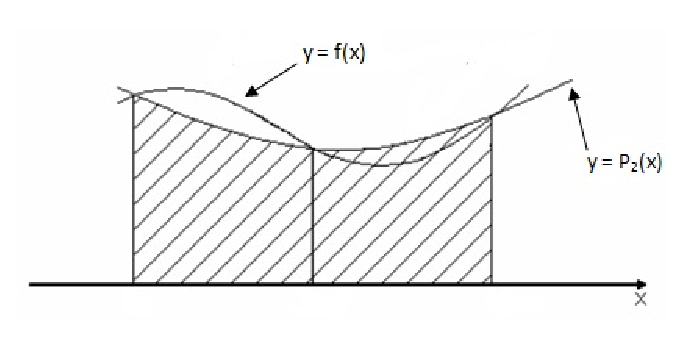
\includegraphics{images/Grafica_Simpson.eps}
  \caption{Descripci�n gr�fica de la regla de Simpson}
  \label{Grafica_Simpson}
\end{figure}

\section{Regla de Simpson}
\label{2:sec:2}
Utilizando una interpolaci�n polinomial de segundo orden que aproxima a la 
funci�n integrando $f(x)$ entre los puntos a y b, se desea aproximar la integral:

FORMULA 1

La interpolaci�n polinomial que se busca es un polinomio de Lagrange de orden 2,
$P_{2}(x)$, tal que, siendo FORMULA 3

FORMULA 4

Sustituyendo en la integral que se quiere calcular, se obtiene:

FORMULA 5

Se toma:

FORMULA 6

Se despeja b de forma que:

FORMULA 7

Se sustituye la expresi�n $(a-c)(a-b)$ de la siguiente forma:

FORMULA 8

Obteni�ndose as� que:

FORMULA 9

Realizando un cambio de variable tal que $u=x-a$:

FORMULA 10

De la misma forma:

FORMULA 11

De lo que se obtiene que:

FORMULA 12

An�logamente se deduce que:

FORMULA 13

Por tanto, se tiene que:

FORMULA 14

Recordando que la expresi�n FORMULA 15 , la expresi�n anterior se puede expresar como:

FORMULA 16

A esta ecuaci�n se le conoce como Regla de Simpson, y al aproximar tiene un error 
asociado tal que:

FORMULA 17

Donde FORMULA 18 y $\xi$ pertenece al intervalo $[a,b]$.

Se observa que el error es proporcional a la cuarta derivada, de lo que se sigue 
que el m�todo de Simpson obtiene soluciones exactas para ecuaciones de tercer grado 
o inferior.

\section{Regla de Simpson Compuesta}
\label{2:sec:3}

En casos donde la Regla de Simpson devuelva un error elevado debido a la excesiva 
amplitud del intervalo $[a,b]$, se utiliza una variaci�n de la Regla de Simpson conocida 
como Regla de Simpson compuesta, que consiste en dividir el intervalo $[a,b]$ en n (par) 
subintervalos iguales de longitud FORMULA 19 , de tal manera que:

FORMULA 20

Dividiendo la integral en n subintervalos:

FORMULA 21

Aplicando la Regla de Simpson a cada subintervalo $(x_i=a+ih ; i=0,1,2,\ldots,n)$ se sigue 
que, para cada $[x_{j-1},x_{j+1}]$ donde $j=1,3,5,\ldots,n-1$, se obtiene que:

FORMULA 22

Con lo que, recordando que FORMULA 23 , la suma de las integrales de todos los 
subintervalos da como resultado:

FORMULA 24

Ecuaci�n a la que se conoce como Regla de Simpson Compuesta, cuyo error se puede 
acotar tal que:

FORMULA 25

%%%%%%%%%%%%%%%%%%%%%%%%%%%%%%%%%%%%%%%%%%%%%%%%%%%%%%%%%%%%%%%%%%%%%%%%%%%%%%%
\chapter{Procedimiento experimental}
\label{chapter:exp}

%%%%%%%%%%%%%%%%%%%%%%%%%%%%%%%%%%%%%%%%%%%%%%%%%%%%%%%%%%%%%%%%%%%%%%%%%%%%%%%
% Chapter 3: Procedimiento experimental 
%%%%%%%%%%%%%%%%%%%%%%%%%%%%%%%%%%%%%%%%%%%%%%%%%%%%%%%%%%%%%%%%%%%%%%%%%%%%%%%

En este apartado se explicar� el procedimiento que se ha seguido para obtener, 
tanto el valor exacto, como el valor aproximado a trav�s de la regla de Simpson,
de la integral definida:

\[ \int_{1}^{3} x^2\ cos\ x\ \text{d}x \]

A continuaci�n se proceder� a la comparaci�n de ambos resultados. 
A modo de curiosidad se aplicar� la regla de Simpson compuesta para observar la 
mejora en la aproximaci�n.
%++++++++++++++++++++++++++++++++++++++++++++++++++++++++++++++++++++++++++++++
\section{Descripci�n de los experimentos}
\label{3:sec:1}

Los experimentos realizados son los siguientes:

\begin{itemize}
 \item Representaci�n gr�fica de la funci�n.
 \item C�lculo del valor exacto de la integral definida.
 \item Comparaci�n grafica. 
 \item Aproximaci�n por la Regla de Simpson.
 \item Aproximaci�n por la Regla de Simpson compuesta.
\end{itemize}

\subsection{Representaci�n gr�fica de la funci�n.}

Se implementa en Python un programa que representa la gr�fica de la funci�n

\begin{equation}
 f(x)=x^2\ cos\ x
 \label{funcion}
\end{equation}

como se puede ver en el ap�ndice~\ref{Apendice1:grafica1}, obteniendo como 
resultado la figura~\ref{grafica1}.

\begin{figure}[h]
  \begin{center}
    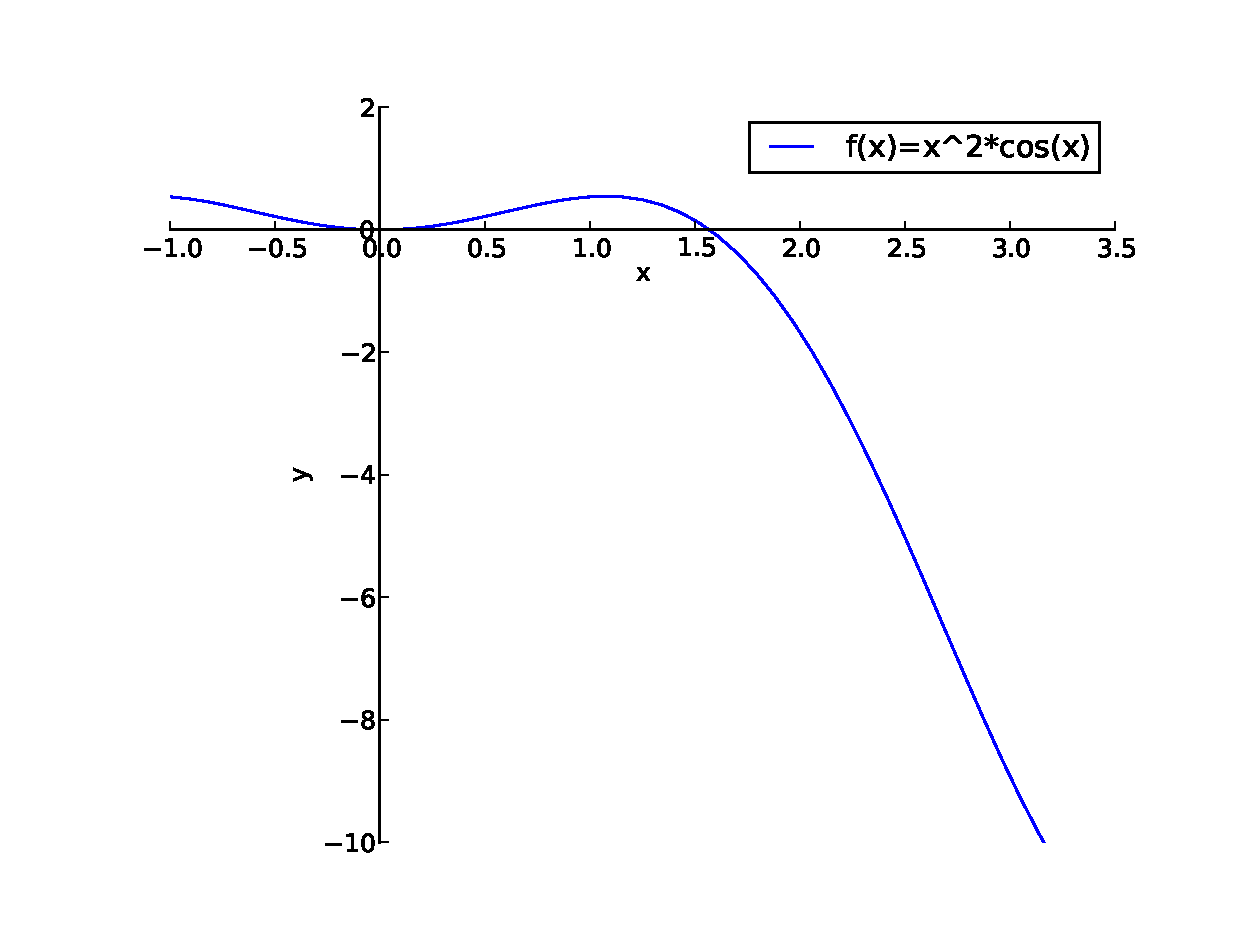
\includegraphics[width=0.75\textwidth]{images/grafica1.eps}
    \caption{Representaci�n gr�fica de la funci�n a integrar.}
    \label{grafica1}
  \end{center}
\end{figure}

\subsection{C�lculo del valor exacto de la integral definida.}

A continuaci�n se detallar�n los pasos seguidos para obtener el valor exacto de la 
integral definida de la funci�n~\ref{funcion} en el intervalo acotado $[1,3]$,
utilizando el segundo teorema fundamental del c�lculo integral (o Regla de Barrow).

Se quiere calcular:

\[ \int_{1}^{3} x^2\ cos\ x\ \text{d}x \]

Primero se resuelve la integral indefinida aplicando el m�todo de integraci�n por 
partes $\left(\int u \text{d}v = uv - \int v \text{d}u\right)$ tal que:
\[ \int x^2\ cos\ x\ \text{d}x =\]\par

\[u=x^2, \quad \text{d}u = 2x\ \text{d}x\] 
\[\text{d}v = cos\ x\ \text{d}x, \quad v = sen\ x \]

Con lo que se obtiene:

\[ \int x^2\ cos\ x\ \text{d}x = x^2 sen\ x - \int 2x sen\ x\ \text{d}x = \]

Empleando de nuevo la integraci�n por partes:

\[ u=2x, \quad \text{d}u = 2\ \text{d}x\]
\[\text{d}v = sen\ x\ \text{d}x, \quad v = -cos\ x \]

Se sigue:

\[ = x^2 sen\ x - \left[-2x cos\ x + 2\int cos\ x\ \text{d}x \right] = 
x^2 sen\ x +2x cos\ x - 2sen\ x = \]

\begin{equation}
 2x cos\ x + (x^2 -2)sen\ x
 \label{primitiva}
\end{equation}

Por �ltimo se obtiene el valor buscado a trav�s de la Regla de Barrow en el 
intervalo $[1,3]$. Para ello se emplear� el lenguaje de programaci�n interpretado
Python, evaluando la expresi�n ~\ref{primitiva}, el resultado se muestra en la 
tabla~\ref{tab:1}, que se encuentra en la p�gina~\pageref{tab:1}.
Se puede ver el c�digo Python en el ap�ndice~\ref{Apendice3:error1} 

\subsection{Comparaci�n gr�fica.}
\begin{figure}[h]
  \begin{center}
    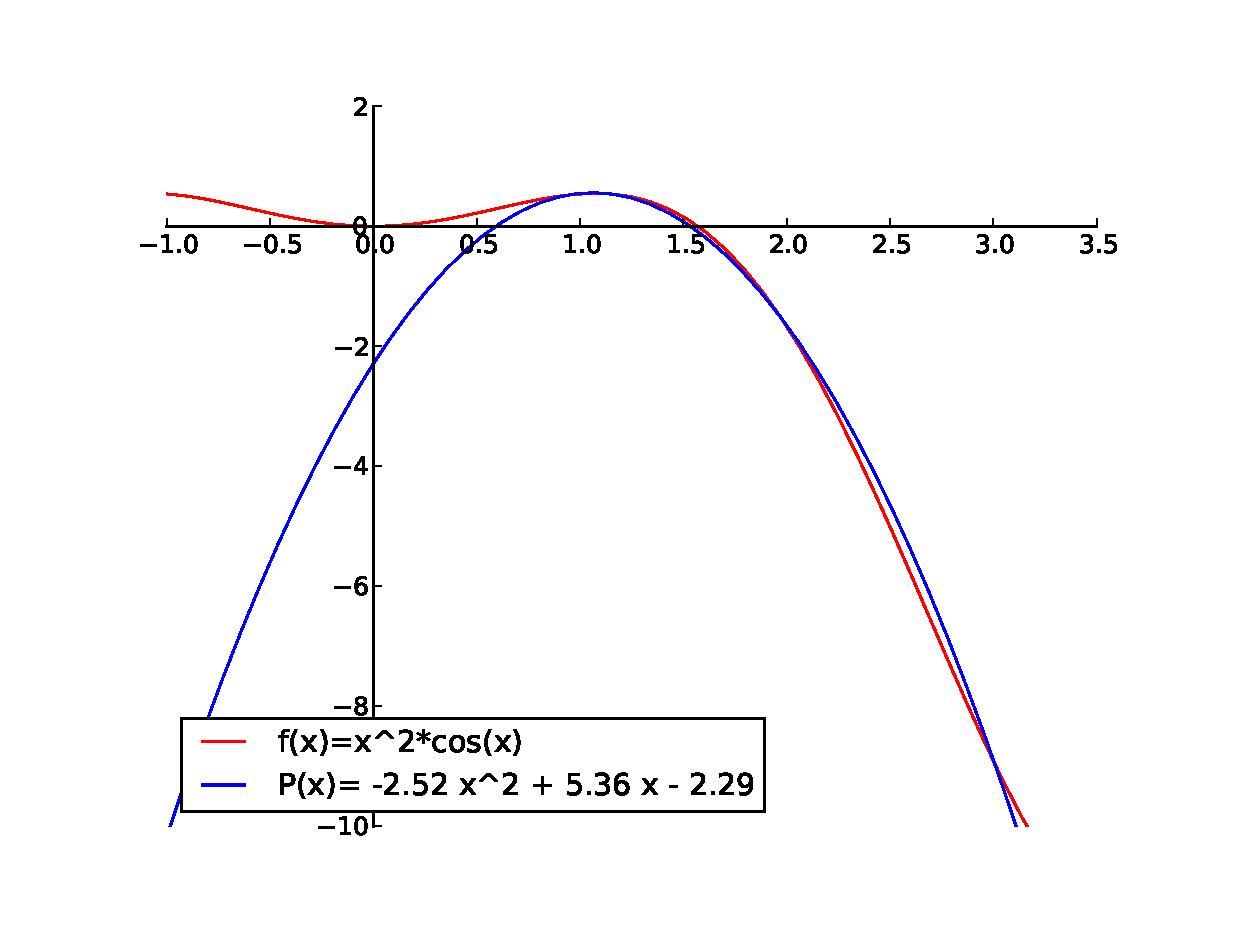
\includegraphics[width=0.75\textwidth]{images/grafica2.eps}
    \caption{Funcion vs. Polinomio interpolador}
    \label{grafica2}
  \end{center}
\end{figure}
En esta secci�n se obtendr� la expresi�n del polinomio interpolador de la regla de Simpson.
Para ello, se busca la expresi�n del polinomio de grado dos que pasa por los puntos 
$(1,f(1)),(2,f(2))\ \text{y}\ (3,f(3))$ de la funci�n~\ref{funcion}.

De esta forma, tenemos:

\[a 1^2 + b 1 + c = f(1)\]
\[a 2^2 + b 2 + c = f(2)\]
\[a 3^2 + b 3 + c = f(3)\]

Obteniendo como resultado:

\begin{equation}
 P_2(x) = -2.520227735 x^2 + 5.355793554 x - 2.295263513
 \label{pol}
\end{equation}

A continuaci�n se implementa en Python un programa que representa la gr�fica $P_2(x)$, frente
a $f(x)$, como se puede ver en el ap�ndice~\ref{Apendice1:grafica2}, obteniendo como resultado 
la figura~\ref{grafica2}.



\subsection{Aproximaci�n por la regla de Simpson.}

Para el c�lculo de una aproximaci�n de la integral:

\[ \int_{1}^{3} x^2\ cos\ x\ \text{d}x \]

se emplea el lenguaje Python, implementando una funci�n que recibe por 
par�metros la expresi�n a estudiar y los extremos del intervalo donde se va a calcular, 
devolviendo la aproximaci�n buscada, el resultado se muestra en la tabla~\ref{tab:1},
que se encuentra en la p�gina~\pageref{tab:1}. Se puede ver el c�digo Python en el 
ap�ndice~\ref{Apendice3:error1}

\subsection{Aproximaci�n por la regla de Simpson compuesta.}

Para un mejor an�lisis de los resultados, se repite el estudio aplicando la Regla de 
Simpson compuesta, implementando una funci�n en Python que recibe por par�metros la expresi�n a estudiar, 
los extremos del intervalo y el n�mero par de subintervalos en los que se ha dividido, devolviendo la 
aproximaci�n buscada, el resultado se muestra en la tabla~\ref{tab:2}, que se encuentra en la 
p�gina~\pageref{tab:2}. Se puede ver el c�digo Python en el ap�ndice~\ref{Apendice3:error2}) 

%++++++++++++++++++++++++++++++++++++++++++++++++++++++++++++++++++++++++++++++
\section{Descripci�n del material}
\label{3:sec:2}
Las caracter�sticas del ordenador empleado para la realizaci�n de este trabajo son las siguientes:
\begin{itemize}
 \item CPU type: Intel(R) Atom(TM) CPU N270   @ 1.60GHz
 \item CPU speed: 800.000Hz
 \item Cache size: 512 KB
\end{itemize}
En cuanto al sistema operativo, se ha utlizado ``Linux-3.2.0-39-generic-i686-with-Ubuntu-12.04-precise''.
Los ficheros en lenguaje Python fueron realizados con el editor de textos avanzado para KDE ``Kate''.

%++++++++++++++++++++++++++++++++++++++++++++++++++++++++++++++++++++++++++++++
\section{Resultados obtenidos}
\label{3:sec:3}

%------------------------------------------------------------------------------
%--------------------------------------------------------------------------
\begin{table}[h]
\begin{center}
\begin{tabular}{|c|c|c|c|} \hline 
\textbf{Valor exacto} & \textbf{Aproximacion} & \textbf{Error absoluto} & \textbf{Error relativo}\\ 
\hline
-5.19124855011 & -5.0093265161 & 0.181922034015 & 0.0350439845558
\\
\hline
\end{tabular}
\end{center}
\caption{Aproximacion y error de la regla de Simpson}
\label{tab:1}
\end{table}


%------------------------------------------------------------------------------
%--------------------------------------------------------------------------
\begin{table}[h]
  \begin{center}
    \begin{tabular}{|c|c|c|c|c|} \hline 
      \textbf{N\'umero de subintervalos} & \textbf{Aproximaci\'on} & \textbf{Error absoluto} & \textbf{Error relativo}\\ 
      \hline
      2 & -5.1817934049 & 0.0094551452 & 0.0018213625
      \\
      \hline
      6 & -5.1911377092 & 0.0001108409 & 0.0000213515
      \\
      \hline
      10 & -5.1912342437 & 0.0000143064 & 0.0000027559
      \\
      \hline
      50 & -5.1912485273 & 0.0000000228 & 0.0000000044
      \\
      \hline
      100 & -5.1912485487 & 0.0000000014 & 0.0000000003
      \\
      \hline
    \end{tabular}
  \end{center}
  \caption{Aproximaci\'on y error de la regla de Simpson compuesta}
  \label{tab:2}
\end{table}


%++++++++++++++++++++++++++++++++++++++++++++++++++++++++++++++++++++++++++++++

\section{An�lisis de los resultados}
\label{3:sec:4}

Como se puede apreciar en la tabla~\ref{tab:1}, el error cometido al emplear la regla de Simpson,
garantiza, para la funci�n estudiada, una precisi�n de por lo menos una cifra decimal exacta.
Por otro lado, se puede observar, que empleando la regla de Simpson compuesta el error es 
inversamente proporcional al n�mero de intervalos, siendo posible reducirlo tanto como se desee.


%%%%%%%%%%%%%%%%%%%%%%%%%%%%%%%%%%%%%%%%%%%%%%%%%%%%%%%%%%%%%%%%%%%%%%%%%%%%%%%
\chapter{Conclusiones}
\label{chapter:conclusiones}

%%%%%%%%%%%%%%%%%%%%%%%%%%%%%%%%%%%%%%%%%%%%%%%%%%%%%%%%%%%%%%%%%%%%%%%%%%%%%
% Chapter 4: Conclusiones y Trabajos Futuros 
%%%%%%%%%%%%%%%%%%%%%%%%%%%%%%%%%%%%%%%%%%%%%%%%%%%%%%%%%%%%%%%%%%%%%%%%%%%%%%%

bla, bla, bla, etc.


%%%%%%%%%%%%%%%%%%%%%%%%%%%%%%%%%%%%%%%%%%%%%%%%%%%%%%%%%%%%%%%%%%%%%%%%%%%%%%%

%%%%%%%%%%%%%%%%%%%%%%%%%%%%%%%%%%%%%%%%%%%%%%%%%%%%%%%%%%%%%%%%%%%%%%%%%%%%%%%
\newpage{\pagestyle{empty}\cleardoublepage}
\thispagestyle{empty}
\begin{appendix}

\chapter{T�tulo del Ap�ndice 1}
\label{appendix:1}

\section{Grafica de la funci\'on}
\label{Apendice1:grafica1}

\begin{center}
\begin{footnotesize}
\begin{verbatim}
###################################################################################
# Fichero: grafica.py
###################################################################################
#
# Contenido: Representacion grafica de la funcion f(x)=x**2*cos(x)
#
# Autor/es: Adrian R. Mendioroz Morales
#           Roberto C. Palenzuela Criado
#
###################################################################################
# Fecha de creacion: 06 de mayo de 2013 
###################################################################################
from math import cos
import matplotlib.pyplot as plt
from matplotlib.ticker import MultipleLocator, FormatStrFormatter
import numpy as np
from matplotlib.pylab import *

def f(t):
  return t**2*cos(t)

t = linspace(-1, 3.5, 51)  # 51 puntos entre 0 y 3
y = zeros(len(t))       # reserva memoria para y con elementos flotantes
for i in xrange(len(t)):
  y[i] = f(t[i])

fig = plt.figure(1)
ax = fig.add_subplot(111) 
# set up axis
ax.spines['left'].set_position('zero')
ax.spines['right'].set_color('none')
ax.spines['bottom'].set_position('zero')
ax.spines['top'].set_color('none')
ax.xaxis.set_ticks_position('bottom')
ax.yaxis.set_ticks_position('left')
 
plot(t,y)
xlabel('x')
ylabel('y')
legend(['f(x)=x^2*cos(x)'],'best')
axis([-1,3.5, -10, 2])  #[tmin, tmax, ymin, ymax]
savefig('grafica.eps')
show()
\end{verbatim}
\end{footnotesize}
\end{center}


\section{Gr\'afica comparativa}
\label{Apendice1:grafica2}

\begin{center}
\begin{footnotesize}
\begin{verbatim}
###################################################################################
# Fichero: grafica2.py
###################################################################################
#
# Contenido: Representacion grafica de la funcion f(x)=x**2*cos(x) y el polinomio
#            de grado 2 que resulta de alicar el metodo de la regla de Simpson.
#
# Autor/es: Adrian R. Mendioroz Morales
#           Roberto C. Palenzuela Criado
#
###################################################################################
# Fecha de creacion: 06 de mayo de 2013 
###################################################################################
from math import cos
import matplotlib.pyplot as plt
from matplotlib.ticker import MultipleLocator, FormatStrFormatter
import numpy as np
from matplotlib.pylab import *

def f1(t):
  return t**2*cos(t)

def f2(t):
  return -2.52*t**2+5.36*t-2.29

t=linspace(-1,3.5,51)
y1 = f1(t)
y2 = f2(t)
  
fig = plt.figure(1)
ax = fig.add_subplot(111) 
# set up axis
ax.spines['left'].set_position('zero')
ax.spines['right'].set_color('none')
ax.spines['bottom'].set_position('zero')
ax.spines['top'].set_color('none')
ax.xaxis.set_ticks_position('bottom')
ax.yaxis.set_ticks_position('left')
 
plot(t,y1,'r')
hold('on')
plot(t,y2,'b')
legend(['f(x)=x^2*cos(x)', 'P(x)= -2.52 x^2 + 5.36 x - 2.29'],'best')
axis([-1,3.5, -10, 2])  #[tmin, tmax, ymin, ymax]
savefig('grafica2.eps')
show()
\end{verbatim}
\end{footnotesize}
\end{center}


\chapter{T�tulo del Ap�ndice 2}
\label{appendix:2}

\section{Modulo Simpson}
\label{Apendice2:Simpson}

\begin{center}
\begin{footnotesize}
\begin{verbatim}
##################################################################################
# Fichero: simpson.py
###################################################################################
# Modulo: Simpson 
#
# Contenido: Funciones de aplicacion de la regla de Simpson de integracion numerica. 
#
# Autor/es: Adrian R. Mendioroz Morales
#           Roberto C. Palenzuela Criado
###################################################################################
# Funciones:
#   regla_simpson: Calcula una aproximacion a la integral de una funcion en un 
#                  intervalo [a,b], aplicando la regla de Simpson.
#      Entrada:
#         f: funcion que se va a aproximar
#         a: limite inferior de integracion
#         b: limite superior de integracion
#      Salida:
#         Aproximacion de la integral de f en [a,b]
# 
#   regla_simpson_compuesta: Calcula una aproximacion a la integral de una funcion en un 
#                            intervalo [a,b], empleando n subintervalos y aplicando la 
#                            regla de Simpson compuesta.
#      Entrada:
#         f: funcion que se va a aproximar
#         a: limite inferior de integracion
#         b: limite superior de integracion
#         n: numero (par) de subintervalos
#      Salida:
#         Aproximacion de la integral de f en [a,b]
###################################################################################
# Fecha de creacion: 06 de mayo de 2013
###################################################################################

from math import *

def regla_simpson(f,a,b):
  return (b-a)/6.0*(f(a)+4*f((a+b)/2.0)+f(b))
  
def regla_simpson_compuesta(f,a,b,n):
  h=(b-a)/float(n)
  aprox=0
  for l in range(0,n):
    aprox+=regla_simpson(lambda x:(x**2*cos(x)),a+l*h,a+(l+1)*h)
  return aprox
\end{verbatim}
\end{footnotesize}
\end{center}



\end{appendix}

%%%%%%%%%%%%%%%%%%%%%%%%%%%%%%%%%%%%%%%%%%%%%%%%%%%%%%%%%%%%%%%%%%%%%%%%%%%%%%%
\addcontentsline{toc}{chapter}{Bibliograf�a}
\bibliographystyle{plain}


\bibliography{bib/references}
\nocite{*}

%%%%%%%%%%%%%%%%%%%%%%%%%%%%%%%%%%%%%%%%%%%%%%%%%%%%%%%%%%%%%%%%%%%%%%%%%%%%%%%

\end{document}
